\chapter{The geometric longitude for strict Conway trees}
\label{app:strict-tree-geometric-characteristic}\label{gj:the-geometric-longitude-for-strict-conway-trees}

A product junction without a crossing circle can be treated geometrically
by inserting a circle around a zero-crossing two-strand box. Filling
that new circle along its meridian removes it and restores the same
ordered tangle. The new circle supplies an angular variable whose
stationary elimination recovers the original product action exactly.

This appendix uses that construction to identify the full preferred
longitude selected by the strict-tree action, including junctions
of arbitrary valence and adjacency. The proof keeps the original
peripheral paths and also covers the possible physical edge label
\(x=1/2\), where an individual edge quadratic has a double root.

\section{The theorem and its geometric conventions}\label{gj:the-theorem-and-its-geometric-conventions}

Use a fixed strict ordered Conway construction from the
\href{https://sashakolpakov.github.io/murakamis_dream/notes/actual_conway_all_strict_tree_long_twist_volume.html}{strict-tree theorem}.
The elementary twist pieces are joined by their prescribed ordered
products and physical quarter-turns, then closed by the original
cylindrical matching. After the forced final product is removed,
strictness means that the real angle domain contains a point with

\begin{equation}\label{gj:T1}
0<a_i<\tfrac12,\qquad
              \max(u,v)<w<u+v<1
\end{equation}

at each original leaf and each retained binary product.
A \emph{bare junction} is a maximal group of consecutive products that
contains no crossing-circle operator. Any binary association used
to calculate it is retained only as an internal resolution;
it does not create additional physical turns.

Require the original strand pairing to give one knot, counting
any circles already closed inside intermediate tangles. Keep all
original parity qualifications. In the two-leaf case retain the
original pure-leaf qualification; the two-odd pairing is a link
and is excluded by the knot test. The construction and
the independently signed twist powers \(n_i\) are fixed before
the quantum level varies. Assume those powers are sufficiently
long for the existing marked strict-tree filling theorem.

A \emph{meridian} goes once around a strand. The \emph{preferred longitude}
follows the knot once and has zero linking number with it.
Holonomy assigns a Möbius transformation to each based closed
path in the complement. We use determinant-one matrix lifts;
\(M\) is the eigenvalue of the positively oriented main meridian,
and \(L\) is the eigenvalue of the preferred longitude on the same
line. The source cut selects the other, \(M^{-1}\), eigenline,
so \(L\) is the inverse longitude eigenvalue on that selected line.

Let \(\mathcal E_T\) be the original physical quarter-turn edges
of the reduced junction tree. On edge \(e\), \(x_e\) is the
normalized polynomial index shared by its two ends after the
trace pairing. When that incidence is exposed as the ordinary
output of the rooted branch, the output angle is \(1-x_e\).
The original ordered construction fixes this convention.
Put \(X_e=e^{2\pi ix_e}\).

\textbf{Theorem.} For every such fixed construction, sufficiently long
independent signed twists give the original complete hyperbolic
knot complement and its regular geometric meridian germ.
On that germ,

\begin{equation}\label{gj:T2}
\boxed{\displaystyle
 L_{\mathrm{geom}}(M)
  =-M^{a(D)}
     \prod_{e\in\mathcal E_T}
       \frac{M^2-X_e(M)}{1-M^2X_e(M)},\qquad
                 a(D)=-w(D)-\sum_i n_i.}
\end{equation}

Here \(w(D)\) is the oriented writhe of the original filled
diagram. The variables \(x_e(M)\) are those of the original
strict-tree stationary action, not those of a different knot
presentation.

More precisely, write \(M=e^{\pi it}\) and let \(\Phi\) be the
original joint first-charge phase at \(M=1\). This is the limiting
logarithmic action of the finite tangle evaluation, with all primitive
filling logarithms retained. Its continued critical point is
defined by

\begin{equation}\label{gj:T3}
\Phi_t=\Phi+
   \sum_{e\in\mathcal E_T}
      \{2J(x_e)-J(x_e+t)-J(x_e-t)\}
                  +\frac{\pi i\,a(D)}2t^2,
 \qquad J'(x)=\log(2\sin\pi x),\quad J(0)=0.
\end{equation}

The theorem identifies this critical branch with the geometric
representation germ of the original filled knot. It identifies
more than its cusp tangent.

At an auxiliary circle the primitive filling slope is
\(\mu_v+p_v\lambda_v\), with original signed crossing power
\(n_v=\epsilon_v-2p_v\). The disk longitude has selected
eigenvalue \(-Q_v\), hence eigenvalue ratio \(Q_v^2\).
A retained half twist means \(\epsilon_v\in\{-1,0,1\}\).
These words and flags are kept in the proof. In particular,
an eigenvalue-ratio equation at \(Q_v=\pm1\) is not used to
discard a possibly nontrivial parabolic filling word.

The \href{https://sashakolpakov.github.io/murakamis_dream/notes/actual_conway_general_mask_marked_filling.html}{marked mask geometry}
supplies the original complete and long-filled holonomies.
The \href{https://sashakolpakov.github.io/murakamis_dream/notes/actual_all_circle_geometric_characteristic.html}{all-circle longitude theorem}
supplies its full rational representation and longitude identity
after circles have been inserted. The argument below connects
the two at the level of ordered group words and of the
\href{https://sashakolpakov.github.io/murakamis_dream/notes/actual_main_meridian_filtered_characteristic.html}{filtered stationary action}.
It imposes no new restriction on bare-junction valence or adjacency
and adds no short-filling quantum claim.

\section{The literal insertion}\label{gj:the-literal-insertion}

Use the reduced tree of original product junctions, with consecutive unturned products already grouped. A bare vertex has full valence at least three. Its incident edges are the original quarter-turns; a binary resolution used to describe its positive kernel does not add physical edges.

At a bare vertex insert the literal unturned box \(R^0=I\), at the distinguished position immediately before the original ordered child product. Encircle its two strands by a new crossing circle. Keep every child in its original order. Put

\begin{equation}\label{gj:1}
\epsilon_v=p_v=n_v=0
\end{equation}

at this new circle. Filling its original primitive meridian removes the auxiliary circle and restores the literal identity box. Thus the filled tangle, its endpoints, its framed main strands and its original peripheral curves are unchanged. No new quarter-turn is inserted. Repeating the operation at all bare vertices produces a literal all-circle tree on the same physical edge set.

\begin{figure}
\centering
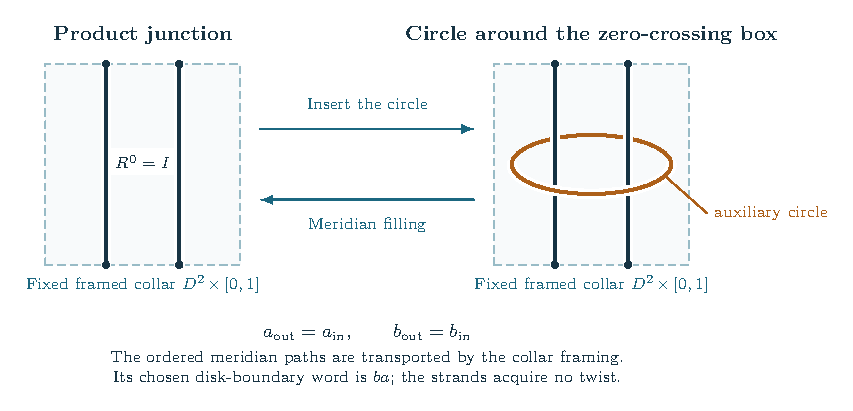
\includegraphics[width=.94\linewidth,keepaspectratio]{../book/figures/zero-circle-junction.pdf}
\caption{A crossing circle is added around two straight strands in a fixed framed collar. Meridian filling removes it. The transported based meridians satisfy \(a_{\mathrm{out}}=a_{\mathrm{in}}\) and \(b_{\mathrm{out}}=b_{\mathrm{in}}\); their chosen disk-boundary word is \(ba\).}
\label{fig:strict-zero-circle-junction}
\end{figure}

The fixed access paths make these ordered equalities precise. They
are constructed in Section~\ref{gj:what-the-edge-equations-see-at-the-complete-bare-representation}; the figure records the collar without
choosing additional paths.

For a holonomy representation, the added meridian must be projectively
identity: its matrix must be a scalar. An eigenvalue ratio of one would
also permit a nontrivial parabolic matrix. Section~\ref{gj:a-unique-regular-zero-power-angular-saddle} excludes this
ambiguity by exhibiting an auxiliary longitude with distinct eigenvalues.

The original crossing powers, writhe and integer

\begin{equation}\label{gj:2}
a(D)=-w(D)-\sum_v n_v.
\end{equation}

are unchanged. The added circles have filling parameter zero, so their preferred-longitude surgery correction \(p_v\ell_v^2\) also vanishes.

\begin{figure}
\centering
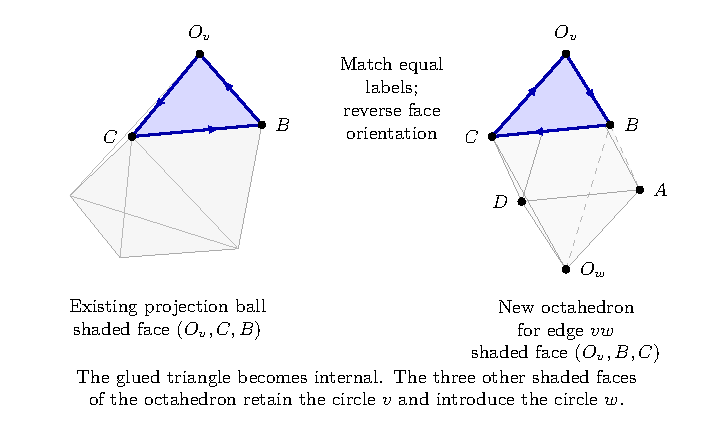
\includegraphics[width=.94\linewidth,keepaspectratio]{../book/figures/octahedral-page-attachment.pdf}
\caption{An ordered page attachment glues an edge block along a shaded triangle, retaining circle v and introducing circle w.}
\end{figure}

After the zero-power circles have been inserted, the
\href{https://sashakolpakov.github.io/murakamis_dream/notes/actual_all_circle_octahedral_decomposition.html}{ordered all-circle cut}
uses this attachment at every tree edge. The labels fix the page order.
The representation comparison below also permits a flat added
subdivision; it uses the original strict geometry to identify the knot
holonomy.

\section{A unique regular zero-power angular saddle}\label{gj:a-unique-regular-zero-power-angular-saddle}

Let a bare hub have \(m\ge3\) incident covariant labels \(x_1,\ldots,x_m\), with

\begin{equation}\label{gj:3}
0<x_j\le\tfrac12,\qquad
 \#\{j:x_j=\tfrac12\}\le1,\qquad
                         \sum_jx_j>1.
\end{equation}

The \href{https://sashakolpakov.github.io/murakamis_dream/notes/actual_main_meridian_component_pressure.html\#4-complete-physical-edge-labels-are-at-most-half}{complete physical-edge theorem}
and the \href{https://sashakolpakov.github.io/murakamis_dream/notes/actual_main_meridian_general_component_comparison.html\#8-the-original-complete-wire-window-and-complex-angular-parameters}{original wire-window argument}
give these conditions at the original complete strict optimizer. All physical labels are strictly below half except for the internal edge of the two-trivalent-hub component; that exception supplies at most one half label to either hub. Strict whole-hub support gives the final inequality. Hidden resolution labels are not included in \eqref{gj:3}.

The angular variable \(\tau\) describes the auxiliary disk longitude
by \(Q=e^{i\tau}\). The
\href{https://sashakolpakov.github.io/murakamis_dream/notes/actual_main_meridian_regular_circle_trace.html}{circle-incidence action}
is

\begin{equation}\label{gj:4}
b(x,\tau)=\int_0^x
       \log(2\cos(2\pi r)+2\cos\tau)\,dr-2J(x),
 \qquad J'(x)=\log(2\sin\pi x).
\end{equation}

Here \(J(0)=0\); its derivative specifies its continued branch. For \(\tau=-iy\), \(y>0\), every logarithm in the integral is real and finite. Put \(k=\tanh(y/2)\). Direct integration gives

\begin{equation}\label{gj:5}
b_\tau(x,-iy)=\frac{i}{\pi}
             \arctan\bigl(k\tan(\pi x)\bigr),
 \quad 0<x<\tfrac12,
\end{equation}

with value \(i/2\) at \(x=1/2\). Indeed
\[
 \int_0^x\frac{\sinh y}{\cosh y+\cos2\pi r}\,dr
   =\frac1\pi\arctan\bigl(k\tan\pi x\bigr).
\]
The zero-power first-charge equation is therefore

\begin{equation}\label{gj:6}
\sum_jb_\tau(x_j,\tau)-i=0
 \quad\Longleftrightarrow\quad
 \sum_j\arctan(k\tan\pi x_j)=\pi.
\end{equation}

A half label contributes \(\pi/2\). The left side is strictly increasing for \(0<k<1\), starts at zero or \(\pi/2\), and tends to \(\pi\sum_jx_j>\pi\). Thus \eqref{gj:6} has exactly one solution \(0<k<1\). Consequently

\begin{equation}\label{gj:7}
y=2\operatorname{arctanh}k>0,\qquad
 Q=e^{i\tau}=e^y=\frac{1+k}{1-k}>1.
\end{equation}

At least two labels are strictly below half. Differentiating \eqref{gj:6} shows that its derivative is strictly positive, so the angular Hessian is nonzero. The saddle and its selected logarithms extend holomorphically to a complex neighborhood of the fixed label tuple. The half-label case causes no singularity: the integrand of \eqref{gj:4} remains nonzero at \(y>0\), and \eqref{gj:6}'s derivative still has the contributions of the other labels.

In particular the new auxiliary longitude has distinct eigenvalues. If its meridian has similarity one and commutes with that longitude, it is projectively identity. The possible unipotent ambiguity at \(Q^2=1\) is absent.

\section{Exact elimination of the angular action}\label{gj:exact-elimination-of-the-angular-action}

Let \(V_m(\mathbf x)\) be the complete positive action of the whole hub.
It is defined by the \href{https://sashakolpakov.github.io/murakamis_dream/notes/actual_main_meridian_component_pressure.html\#1-complete-actions-boundary-variables-and-product-junctions}{ordered product kernel}: resolve the original ordered product by any fixed binary association, sum its cubic gate actions, and optimize the hidden complementary labels. The conditional optimizer is strict and has negative definite Hessian on the strict whole-hub support.

Then on \eqref{gj:3},

\begin{equation}\label{gj:8}
V_m(\mathbf x)=
 \underset{\tau}{\operatorname{stat}}
       \left\{\sum_jb(x_j,\tau)-i\tau\right\},
 \qquad \tau=-iy \text{ from (6)}.
\end{equation}

The equality includes its constant.

Here is one derivation retaining the exact complete normalization. The Newton factors are the finite polynomial basis used for the
tangle evaluation. For a factor with normalized index \(0<x<1/2\),
the logarithm of its Laurent coefficient at normalized exponent \(r\),
divided by the level, has rate

\begin{equation}\label{gj:9}
B_x(r)=J(2x)-2J(x)-J(x+r)-J(x-r),\qquad |r|\le x.
\end{equation}

The complete trace of a product has first Fourier charge one with coefficient exactly one. Its higher charges have strictly smaller rate; this follows from strict concavity of the positive coefficient convolution, or directly from the \href{https://sashakolpakov.github.io/murakamis_dream/notes/actual_main_meridian_regular_bare_trace.html}{regular bare-trace theorem}. The same exact complete trace is the positive binary-resolution sum. Therefore its rate is both \(V_m(\mathbf x)\) and

\begin{equation}\label{gj:10}
\max_{\substack{\sum_jr_j=1\\ |r_j|\le x_j}}
                               \sum_jB_{x_j}(r_j).
\end{equation}

The two expressions evaluate the same finite polynomial trace. Their
equality determines the local action with its constant and uses no
global quantum-volume asymptotic.

For \(0<x<1/2\),
\[
 B_x'(r)=\log\frac{\sin\pi(x-r)}{\sin\pi(x+r)}.
\]
The unique maximizer of \(B_x(r)+yr\) is

\begin{equation}\label{gj:11}
r=\frac1\pi\arctan\bigl(\tanh(y/2)\tan\pi x\bigr).
\end{equation}

Moreover

\begin{equation}\label{gj:12}
b(x,-iy)=\max_{|r|\le x}\{B_x(r)+yr\}.
\end{equation}

To verify the constant, at \(y=0\) both sides are
\(J(2x)-4J(x)\). Their \(y\)-derivatives are the same \(r\) by \eqref{gj:5} and \eqref{gj:11}. The constrained maximizer \eqref{gj:10} has common multiplier \(y>0\), determined by \(\sum r_j=1\). Equations \eqref{gj:10}--\eqref{gj:12} prove \eqref{gj:8}. A half label follows by continuity. Equivalently \(B_{1/2}(r)=0\), so its tilted maximum is \(y/2\), as also follows directly from \eqref{gj:4}.

For a cubic vertex one can avoid the finite trace altogether. The old action is

\begin{equation}\label{gj:13}
t(x_1,x_2,x_3)=
 \sum_{i<j}J(x_i+x_j)-\sum_iJ(x_i)-J(x_1+x_2+x_3-1).
\end{equation}

Writing \(a_j=\tan\pi x_j\), equation \eqref{gj:6} gives
\(k^2=(a_1+a_2+a_3)/(a_1a_2a_3)\).
The derivative of the right side of \eqref{gj:8} in \(x_j\) is

\begin{equation}\label{gj:14}
\log\frac{\cosh y+\cos2\pi x_j}{2\sin^2\pi x_j}
   =\log\frac{k^2+\cot^2\pi x_j}{1-k^2},
\end{equation}

which is exactly \(\partial_jt\). As \(\sum x_j\downarrow1\), \(y\to\infty\), and both actions tend to \(-2\sum_jJ(x_j)\). This proves the cubic identity with its absolute constant.

Both sides of \eqref{gj:8} are holomorphic near the fixed strict tuple. Their equality on an open real set proves equality of the continued germs. At the possible half label, use their holomorphic continuation from labels below half; both Hessians remain invertible there.

\section{The actual added longitude in the old prism geometry}\label{gj:the-actual-added-longitude-in-the-old-prism-geometry}

The previous section identifies actions. The following matrix calculation identifies the new circle inside the
original marked geometry. A white map is the full Möbius transition
between a white face in one projection copy and its partner in the
other copy. Its translation as well as its fixed points is retained.

In an ordinary output port of the bare product write
\[
 E=e^{2\pi ib},\qquad R=\frac1{1+\kappa},\qquad
 \kappa=e^{-f'(b)}.
\]
The \href{https://sashakolpakov.github.io/murakamis_dream/notes/actual_conway_general_mask_marked_filling.html\#4-actual-and-virtual-white-maps-for-every-mask}{marked product construction}
gives the universal white maps

\begin{equation}\label{gj:15}
W_1=\begin{pmatrix}1&E-1\\0&E\end{pmatrix},\qquad
 W_3=\begin{pmatrix}R&0\\1-E&ER\end{pmatrix}.
\end{equation}

They are the actual top and bottom white-face maps at an unmasked bare product. Through every original binary product, the full matrix identities give

\begin{equation}\label{gj:16}
W_{F,1}=W_{G,1}=W_{o,1},\qquad
 W_{F,3}=W_{G,3}=W_{o,3}
\end{equation}

in the original world frame. Consequently the same ordered side word is seen at every port of that hub.

Insert the zero-crossing box in the original disk frame. Its primitive disk-longitude path crosses these two white sides, giving \(W_1^{-1}W_3\), up to the inversion required when the circle's orientation is reversed. The determinant-one normalization is

\begin{equation}\label{gj:17}
P=\frac1R W_1^{-1}W_3,\qquad
 \operatorname{tr}P
   =2-\frac{4\sin^2\pi b}{R}.
\end{equation}

This is the same \(W_1^{-1}W_3\) disk word used at the corresponding end of an all-circle edge; it is not a trace chosen to fit \eqref{gj:6}.

The response metric records the ordered quadrilateral shape at a
product boundary. Its coordinate \(X_{\mathrm{met}}\) is distinct
from the exponential wire variable \(X_e=e^{2\pi ix_e}\). It is
\[
 X_{\mathrm{met}}^2=\frac{1+\cot^2\pi b}{1+\kappa}.
\]
Therefore

\begin{equation}\label{gj:18}
\operatorname{tr}P=2-\frac4{X_{\mathrm{met}}^2}.
\end{equation}

At a boundary incidence with covariant label \(x\), the ordinary output is \(b=1-x\), and the conditional action satisfies \(f'(b)=-\partial_xV_m\). Using \eqref{gj:14}, valid at any valence by the envelope identity \eqref{gj:8}, gives

\begin{equation}\label{gj:19}
X_{\mathrm{met}}^2
 =\frac1{\sin^2\pi x\,[1+\exp(\partial_xV_m)]}
 =\operatorname{sech}^2(y/2)=1-k^2.
\end{equation}

Thus

\begin{equation}\label{gj:20}
\operatorname{tr}P=-2\cosh y=-(Q+Q^{-1}).
\end{equation}

This proves that the actual added longitude has the regular eigenvalues required by the angular saddle. The proof retains the old group word, and shows why a bare hub has a common \(Q\) across all its pages.

When an incidence is viewed through its physical turn, the old identity
\(T W_{j+1}(E,R)=W_j(E^{-1},1-R)T\)
takes the \(W_1^{-1}W_3\) word to the appropriate inverse of the \(W_2^{-1}W_0\) word. Its trace is unchanged. The auxiliary flag may be selected on the eigenvalue \(-Q\), \(Q>1\); the main meridian flags are not changed by this auxiliary choice.

\section{What the edge equations see at the complete bare representation}\label{gj:what-the-edge-equations-see-at-the-complete-bare-representation}

Pull the original complete holonomy back along the exact filling quotient obtained in Section~\ref{gj:the-literal-insertion}. This gives a representation of the enlarged augmented link with every newly added meridian equal to identity. It is a representation-theoretic pullback; no assertion that the drilled link carries this metric is needed.

\subsection{The marked zero-crossing collar}\label{gj:the-marked-zero-crossing-collar}

Choose the box in a framed ball \(D^2\times[0,1]\), with its two strands
\(\{p_1,p_2\}\times[0,1]\). Choose a basepoint \(z_*\in\partial D^2\),
an ordered pair of disjoint access paths from it to small circles around
\(p_1,p_2\), and transport that entire system by the product framing.
Orient and name the resulting based puncture loops \(a,b\) so that
the oriented disk-boundary word is \(ba\). The boundary basepath is
\(\{z_*\}\times[0,1]\). Transport across this literal zero-crossing box gives

\begin{equation}\label{gj:22c}
a_{\mathrm{out}}=a_{\mathrm{in}},\qquad
                        b_{\mathrm{out}}=b_{\mathrm{in}}.
\end{equation}

These are equalities in the based fundamental group, before taking any
representation. No permutation of punctures, turn of an access path,
or power of the disk-boundary curve is included.

Place the new auxiliary circle at the disk boundary in the middle
of this collar, with the original disk framing. Its longitude is
the parallel copy of that boundary and retains the based word \(ba\).
The meridian filling deletes the auxiliary circle and returns exactly
the framed collar just described. Its quotient on fundamental groups
fixes \(a,b\), their access paths, and the boundary basepath. Thus it
also fixes the ordered maps by which this collar is joined to all
earlier and later product factors. This remains true when there are
several child factors: transport the same system through them in
their recorded order. It never requires the factors to commute.

For comparison with a pair of projection faces, transport the framed
loops to the face basepoints along the original specified paths.
If the old transport is \(C_0\), \eqref{gj:22c} becomes the simultaneous
conjugacy \(C_0aC_0^{-1}=a'\), \(C_0bC_0^{-1}=b'\).
Reading the other side of a puncture changes the corresponding
native generator to its inverse. Those inversions are recorded
explicitly in \eqref{gj:22b} below; they do not change \eqref{gj:22c} into a braid.
This is the marked van Kampen statement used at every added seam.
Only a retained nonzero half twist changes \eqref{gj:22c}, by the separately
calibrated Hurwitz action.

A port here is the ordered quadrilateral chart supplied by the
original cell construction. It is not assumed to be a new
four-punctured topological boundary. On a physical turn edge use its
original coordinate \((0,\infty,1,R)\) and its phase \(E=e^{2\pi ix}\).
This is the transported physical-edge frame from the last paragraph
of Section~\ref{gj:the-actual-added-longitude-in-the-old-prism-geometry}; its phase is the reciprocal of the ordinary-output
phase \(e^{2\pi ib}\), with the corresponding change \(R\mapsto1-R\).
At \(M=1\) the four \href{https://sashakolpakov.github.io/murakamis_dream/notes/actual_all_circle_geometric_characteristic.html\#2-the-local-face-maps}{native all-circle white matrices} are exactly the universal old \(W_j(E,R)\), projectively. This follows by putting \(m=1\) in the explicit native chart, without specializing the auxiliary eigenvalues to one.

The two disk words have normalized traces \(-\beta,-\gamma\), where

\begin{equation}\label{gj:21}
\beta=\frac{2R-(E+E^{-1})}{1-R},\qquad
 \gamma=\frac{2-(E+E^{-1})-2R}{R}.
\end{equation}

At an inserted hub these are supplied by \eqref{gj:20}; at an original circle they are its original marked longitude trace. Eliminating \(R\) yields

\begin{equation}\label{gj:22}
A=\frac{4-\beta\gamma}{\beta+\gamma+4},
 \qquad A=E+E^{-1},
\end{equation}

which is exactly the all-circle edge equation at \(M=1\). Thus the old phase is one of its two reciprocal roots. The native white maps retain \(E\) itself, not just \(E+E^{-1}\); the existing native/character comparison identifies the all-circle source variable with that \(E\).

All character-chart denominators are units at this point: \(\beta,\gamma\ge2\), \(E\ne1\), and the displayed original port vertices are distinct. The allowed value \(E=-1\) on the two-hub half edge does not cause a character-matrix singularity. In that case the edge quadratic may ramify over its endpoint parameters; one must use the full stationary branch or another local coordinate, not assert that \(E\) is a simple quadratic root.

Indeed \(E=-1\) gives

\begin{equation}\label{gj:22e}
(\beta-2)(\gamma-2)=16
 \quad\Longleftrightarrow\quad
 X_{\mathrm{met},v}^{\,2}+X_{\mathrm{met},w}^{\,2}=1,
\end{equation}

by \eqref{gj:18}. This is the possible half-edge fold of the old geometry.
The normalized matrices and the two irreducible puncture pairs
below remain regular there.

Here is the boundary-group comparison, including the tuple that has to be retained. First choose the normalized native matrix representatives for the four old projective white maps. In terms of the raw universal representatives used in \eqref{gj:15}, their scalar factors are respectively

\begin{equation}\label{gj:22d}
E^{-1},\quad E^{-1},\quad
                [E(1-R)]^{-1},\quad (ER)^{-1}.
\end{equation}

Each normalized matrix has determinant \(E^{-1}\) at \(M=1\).
The raw universal representatives do not all have that determinant:
in particular the factors involving \(R\) and \(1-R\) cannot be
discarded when taking an SL trace. With \(W_j\) now denoting these
normalized native representatives, put in each original edge frame

\begin{equation}\label{gj:22a}
N_j=W_{j-1}^{-1}W_j,\qquad
 (A,B,C,D)=(N_3,N_0,N_1,N_2)
\end{equation}

with the subsequent determinant-one puncture normalizations from the
all-circle chart. These subsequent powers of \(M\), not the scalar
factors in \eqref{gj:22d}, are one at \(M=1\). Thus every \(N_j\) has determinant
one and trace two. The actual page table is

\begin{equation}\label{gj:22b}
\begin{array}{c|c|c|c}
\text{end}&(a,b)&(a',b')&ba=b'a'\\ \hline
v&(B,A)&(C^{-1},D^{-1})&AB\\
w&(B^{-1},C^{-1})&(A,D)&(BC)^{-1}.
\end{array}
\end{equation}

The entries refer to paths, with the inverse on each puncture determined by its side of the disk. They are exactly the table of the literal all-circle cut, not a new identification of equal traces.

To apply that table to the old holonomy, first insert the zero-crossing box in the actual diagram, before assigning matrices. The main strands and their ordered endpoint paths are unchanged. Add the new circle and perform the literal projection/disk cut. The filling quotient takes every old main meridian and its old basepath to itself and kills the new circle meridian. In particular the four small corner paths reduce to the original consecutive-white words in \eqref{gj:22a}. A white face split by the added cut retains the same transport on both of its pieces: crossing the extra cut and returning differs by the new meridian, whose image is identity. This is also the full-map invariant \eqref{gj:16} through every prism of the original product. Thus the developed four white transitions of the pulled-back representation are exactly the four \(W_j\) already compared above.

The paths across the added disk pages are still the paths of this cut. By van Kampen they intertwine both generators in the appropriate row of \eqref{gj:22b}, with precisely the displayed inversions; the product column is their original primitive disk boundary. The inserted box has no crossing, so no Hurwitz exchange is made at its distinguished seam. The old retained half twists keep their original exchanges.

At \(M=1\), either input pair in \eqref{gj:22b} is irreducible. Both punctures have trace two, and the products in the two rows have traces \(-\beta\) and \(-\gamma\), respectively, with \(\beta,\gamma\ge2\). Their irreducibility obstructions are \((\beta+2)^2\ne0\) and \((\gamma+2)^2\ne0\). Two intertwiners of either full ordered pair differ by its scalar centralizer. Therefore the pulled-back page transport equals the native pure transport in PGL. At an original odd seam the same argument is applied after the already calibrated full Hurwitz action. The corner flags on the main cusp are the old parabolic flags, and the extra auxiliary flags are chosen from \eqref{gj:20}; these choices do not alter a group generator.

All white and shaded generators of the cut now agree, in their original tree frames. This proves equality of the complete representations, not only of the local character triples or the main-cusp translation. It identifies the selected all-circle algebraic point with the pullback of the original bare-tree holonomy. The newly introduced ideal vertices need not form positive tetrahedra in this pulled-back representation. In particular an edge with \(E=-1\) can make that added subdivision flat. No metric on the enlarged unfilled exterior is asserted or required.

\section{Stationary elimination at a nonparabolic main meridian}\label{gj:stationary-elimination-at-a-nonparabolic-main-meridian}

Let \(t\) be the actual main deformation parameter, \(M=e^{\pi it}\).
In the existing strict-tree filtered action it enters only through

\begin{equation}\label{gj:23}
\sum_{e\in\mathcal E_T}
       \{2J(x_e)-J(x_e+t)-J(x_e-t)\}
       +\frac{\pi i a(D)}2t^2.
\end{equation}

It does not enter the old bare tensor action or its hidden resolution wires.

The enlarged all-circle action replaces a bare hub by
\(\sum_jb(x_j,\tau_v)-i\tau_v\), with \(n_v=0\).
Eliminating \(\tau_v\) by \eqref{gj:8} returns exactly the old whole-hub action, including its constant, for complex physical wires in the regular neighborhood. The edge set and \eqref{gj:23} do not change, and neither does \(a(D)\). Hence the two full critical-value germs are equal after stationary elimination.

The new angular Hessian at each bare hub is nonzero. To state the
comparison precisely, first eliminate the old hidden binary-resolution
variables. Their conditional Hessian is invertible by strictness.
Let \(z\) collect the remaining original variables and let
\(\tau_{\mathrm{new}}\) collect only the added angular variables.
The enlarged Hessian has blocks

\begin{equation}\label{gj:23a}
H_{\mathrm{new}}=
 \begin{pmatrix}
 H_{zz}&H_{z\tau}\\ H_{\tau z}&H_{\tau\tau}
 \end{pmatrix},\qquad
 H_{\mathrm{old,red}}
   =H_{zz}-H_{z\tau}H_{\tau\tau}^{-1}H_{\tau z}.
\end{equation}

The block \(H_{\tau\tau}\) is diagonal over the added hubs, with
nonzero entries from \eqref{gj:6}. Equality \eqref{gj:8} identifies its Schur
complement with the old reduced Hessian. The original full Hessian
and its eliminated hidden block are invertible, so
\(\det H_{\mathrm{new}}
 =\det H_{\tau\tau}\det H_{\mathrm{old,red}}\ne0\).
No individual edge Hessian is inverted, including at \eqref{gj:22e}.

The enlarged analytic branch therefore exists with all the original
logarithms retained. Original sufficiently long fillings keep their
auxiliary \(Q_v^2\ne1\); every added zero-power circle has
\(Q_v^2\ne1\) by \eqref{gj:7}, and this persists near the complete branch.

By Section~\ref{gj:what-the-edge-equations-see-at-the-complete-bare-representation} this branch reconstructs the original filled knot representation, rather than only an algebraic solution of the slope eigenvalue equations. Near the old augmented complete point the original auxiliary deformation is fixed by its primitive peripheral rows. Equality at completeness and the marked gluing/representation local inverse identify the two nearby deformations. The original sufficiently long filling point lies on that same small branch. There every original filled circle, as well as every added zero circle, has \(Q_v^2\ne1\); the filling words are projectively identity by Section~\ref{gj:a-unique-regular-zero-power-angular-saddle}. The nondegenerate main-meridian branch is then the geometric germ of the original filled knot.

The all-circle squared longitude identity is a rational identity on its integral source variety. It extends to this regular representation, including the half-edge fold, without solving for an individual edge root. The added zero fillings contribute no surgery exponent, the Seifert sign is that of the same original complete knot, and stationary elimination leaves the effective longitude unchanged. Consequently

\begin{equation}\label{gj:24}
L_{\mathrm{geom}}(M)
   =-M^{a(D)}
      \prod_{e\in\mathcal E_T}
                \frac{M^2-X_e(M)}{1-M^2X_e(M)}
\end{equation}

on the original strict-tree filled branch, with \(X_e=e^{2\pi ix_e}\).

This proves the theorem on the geometric germ of the original
filled knot. The same physical edges occur before and after the
zero-circle elimination, and the added circles contribute neither
a crossing power nor a preferred-longitude shear.

The geometric identification uses the full ordered boundary-group
comparison in Section~\ref{gj:what-the-edge-equations-see-at-the-complete-bare-representation}. The equality of actions in Section~\ref{gj:exact-elimination-of-the-angular-action} supplies
the stationary branch, while the marked face maps identify its
representation. These are distinct parts of the proof. The established
strict-tree quantum estimates retain their existing long-filling
hypotheses; this argument adds no estimate for short fillings.

\section{The geometric factor selected by the actual recurrence}\label{gj:the-geometric-factor-selected-by-the-actual-recurrence}

The geometric theorem identifies the curve already selected by the
full asymptotic expansion of the original strict-tree invariant.
This extends the operator consequence beyond trees whose junctions
all carry crossing circles. It requires no quantum estimate for the
newly drilled diagram: the quantum source remains the original
strict presentation.

Fix an oriented strict ordered Conway knot presentation \(D\), with
its original cut, endpoint orders, framing and signed integral
crossing powers. Assume the powers are independently sufficiently
long for the \href{https://sashakolpakov.github.io/murakamis_dream/notes/actual_main_meridian_filled_volume.html}{filled-meridian theorem}
and the geometric theorem above. The entire diagram and every power
are fixed before \(N\) tends to infinity. All original knot-pattern
and absence-of-internal-component qualifications remain in force.
Both level parities and all sufficiently large composite levels are
included.

Write \(F_N(M)\) for the actual zero-framed reduced ADO invariant,
with

\begin{equation}\label{gj:O1}
q_N=e^{\pi i/N},\qquad M=-q_Nx,\qquad F_N(1)=K_N(K).
\end{equation}

Here \(x\) is the raw highest-weight parameter, distinct from an
internal normalized index \(x_e\). The marked complete meridian is
\(M=1\), and \(X_e=e^{2\pi ix_e}\) denotes the original physical-edge
variable.

Let

\begin{equation}\label{gj:O2}
P(q,M,T)=\sum_{j=0}^{d}a_j(q,M)T^j,\qquad
 a_j\in\mathbb C(q,M),\qquad TM=qMT,
\end{equation}

be any specified nonzero fixed operator that annihilates the whole
function \(F_N(M)\) at every sufficiently large level. The shift \(T\)
replaces \(M\) by \(qM\). Such an actual all-level annihilator exists
by the \href{https://sashakolpakov.github.io/murakamis_dream/notes/finite_sum_annihilator.html}{finite-sum construction}; it is not
defined by fitting the complete values or adjoining a desired factor.
An operator with negative shift powers can first be multiplied by
a power of \(T\).

Clear fixed rational denominators, remove the common \(q-1\)
valuation of the coefficients, and denote the resulting first nonzero
classical symbol by \(P_0(M,L)\). Let
\(A_{\mathrm{geom},\mathbb C}(M,L)\) generate the Laurent prime of the
actual geometric eigenvalue germ through \((1,-1)\), in the preferred
meridian and longitude of the original knot. The longitude coordinate
is its eigenvalue on the \(M\) line, equivalently the inverse
eigenvalue on the source \(M^{-1}\) line.

Then

\begin{equation}\label{gj:O3}
\boxed{\displaystyle
 A_{\mathrm{geom},\mathbb C}(M,L)\mid P_0(M,L)
 \quad\text{in }\mathbb C[M^{\pm1},L^{\pm1}].}
\end{equation}

Thus every genuine all-level annihilator has the same selected
irreducible geometric factor in its first classical symbol.

\subsection{Proof and normalization}\label{gj:proof-and-normalization}

The \href{https://sashakolpakov.github.io/murakamis_dream/notes/actual_main_meridian_filtered_characteristic.html}{filtered characteristic theorem},
Sections 2--6, already applies to the full strict long-filling class,
including arbitrary bare components. It proves the complete
microscopic expansion with its degree filtration on all the finitely
many translated parameter charts needed by \eqref{gj:O2}. This shifted-chart
statement follows from the exact source and its endpoint estimates,
not from continuation of an asymptotic formula on a single disk.

The normalized full state is

\begin{equation}\label{gj:O4}
\mathcal Z_N(s)=\frac{F_N(q_N^s)}{F_N(1)H_N(s)},\qquad
 H_N(s)=\frac{\sin\pi s}{N\sin(\pi s/N)}.
\end{equation}

It retains the exact modified-dimension gauge

\begin{equation}\label{gj:O5}
d_N(M)=\eta_N\frac{M-M^{-1}}{M^N-M^{-N}},\qquad
 d_N(1)=\eta_N/N,\qquad
 \frac{d_N(q_N^s)}{d_N(1)}=H_N(s)^{-1}.
\end{equation}

Here \(\eta_N=i^{N+3}\). Put \(f(M)=M-M^{-1}\). The operator on the
full state has shift coefficients

\begin{equation}\label{gj:O6}
\widetilde a_j(q,M)
 =a_j(q,M)(-1)^j\frac{f(M)}{f(q^jM)}.
\end{equation}

Multiplication on the left by \(\prod_{j=1}^{d}f(q^jM)\)
gives the first classical symbol \(f(M)^dP_0(M,-L)\). The meridian
divisor and shift sign are therefore retained before the formal cancellation.

The filtered theorem defines the selected critical value \(S(t)\)
using the original phase and the insertion

\begin{equation}\label{gj:O7}
\sum_{e\in\mathcal E_T}
 [2J(x_e)-J(x_e+t)-J(x_e-t)]
 +\frac{\pi i a(D)}2t^2.
\end{equation}

Its expansion has coefficient of order \(N^{-r}\) of degree at
most \(r+1\) in \(s\). The top-degree coefficients come from \(S\);
lower Gaussian amplitudes cannot change them. With
\(\mathcal S(u)=\pi i[S(u/(\pi i))-S(0)]\), the exact operator
equation and this filtration give the formal domain identity

\begin{equation}\label{gj:O8}
f(e^u)^dP_0(e^u,-e^{\mathcal S'(u)})=0.
\end{equation}

The full argument, including injectivity of the substitution
\(u=hs\), is in
\href{https://sashakolpakov.github.io/murakamis_dream/notes/actual_all_circle_geometric_characteristic.html\#11-the-geometric-factor-of-an-actual-quantum-recurrence}{the all-circle operator proof},
Section~\ref{gi:all-orders-shifted-charts-and-the-geometric-branch}. That argument depends on the filtered source expansion
and the exact gauge, not on the absence of bare vertices. The
nonzero series \(f(e^u)^d\) can be cancelled in this proved integral
domain identity.

The new geometric input identifies its entire selected germ:

\begin{equation}\label{gj:O9}
-e^{\mathcal S'(\log M)}
 =-M^{a(D)}\prod_{e\in\mathcal E_T}
              \frac{M^2-X_e(M)}{1-M^2X_e(M)}
 =L_{\mathrm{geom}}(M).
\end{equation}

The zero-circle elimination above preserves the whole critical-value
germ and the original physical-edge set. Its ordered boundary-group
anchor identifies the original filled geometric representation.
The preferred-longitude sign is fixed at that filled knot point.
Thus \eqref{gj:O9} is not inferred from the cusp tangent or from a choice among
unmarked exponentiated solutions.

It follows that \(P_0\) vanishes on the geometric eigenvalue germ.
Its Laurent evaluation kernel is a nonzero prime and contains no
nonzero polynomial in \(M\) alone, because \(M\) varies. It is
therefore a height-one prime in a Laurent polynomial unique
factorization domain, proving \eqref{gj:O3}.

If the operator coefficients lie in \(\mathbb Q(q,M)\), contract
that same germ prime to \(\mathbb Q[M^{\pm1},L^{\pm1}]\). Its
irreducible generator divides the rational symbol. Its complex
factorization contains the selected geometric factor and any
conjugate factors required over \(\mathbb Q\); an individual complex
component need not itself be defined over \(\mathbb Q\).

\section{Transfer to presentations with net twists and arbitrary closures}\label{gj:transfer-to-presentations-with-net-twists-and-arbitrary-closures}

The conclusion is intrinsic to the zero-framed knot with its marked
peripheral curves. Suppose the
\href{https://sashakolpakov.github.io/murakamis_dream/notes/actual_conway_net_twist_volume.html}{ordered net-twist reduction} gives
an actual ambient isotopy from the input knot to a strict knot
presentation covered by Section~\ref{gj:the-geometric-factor-selected-by-the-actual-recurrence}. The isotopy carries the knot
orientation, meridian, preferred zero-linking longitude and cut mark.
Correcting any transported ribbon framing to zero gives exactly the
same reduced ADO function \(F_N(M)\) at every level and every
meridian value where it is defined. Its rational continuation is
therefore the same function as well.

The geometric eigenvalue germ is also the same under this marked
isotopy. An actual all-level operator for the input family thus
satisfies the hypotheses of Section~\ref{gj:the-geometric-factor-selected-by-the-actual-recurrence} for that same intrinsic
family. Its first classical symbol contains the selected geometric
factor. This transfers the factor statement without identifying
presentation-specific recurrence formulas or their unreduced
polynomial representatives.

The same argument applies to the
\href{https://sashakolpakov.github.io/murakamis_dream/notes/actual_conway_arbitrary_closure_volume.html}{arbitrary-closure reduction}
when its hypotheses yield one covered strict knot factor and only
unknot factors. In particular, under its long surviving-factor
hypotheses, a hyperbolic knot input has exactly that form. Removing
the exhibited unknot summands is an actual orientation-preserving
ambient isotopy. The preferred peripheral pair is carried by the
induced map of exteriors. No multiplicativity assertion for quantum
growth over connected sums is required.

For a fixed original expression there are finitely many recorded
reduction and parity branches. If a uniform net-weight statement is
desired, take the maximum of the strict source and geometric
thresholds over those finitely many possible strict outputs. The
threshold concerns their surviving signed net powers. Large
individual powers that cancel to a short surviving power do not
satisfy it. This does not assert that an earlier, smaller
complete-value threshold automatically supplies the stronger
moving-meridian hypotheses.

The integer \(a(D)\) and the individual edge factors in \eqref{gj:O9} are
computed on the covered strict diagram. They are not claimed to
equal those read from an unreduced input presentation term by term.
The preferred geometric longitude and its selected irreducible
factor are the intrinsic objects that transfer.

The conclusions concern one irreducible geometric factor, not the
full A-polynomial, its multiplicity, or an equality of quantum
operator ideals. They do not provide a fixed-\(M\) large-level WKB
theorem, nonvanishing through ordinary-color resonances, or a
general short-twist theorem. The wider quantitative all-circle
alternatives remain available under their own source and geometric
hypotheses; this section neither narrows those results nor extends
them to arbitrary short bare-junction fillings.
